\documentclass[11pt,landscape,a4paper,fleqn]{article}
\usepackage[utf8]{inputenc}
\usepackage[ngerman]{babel}
\usepackage{tikz}
\usepackage{bbm}
\usetikzlibrary{shapes,positioning,arrows,fit,calc,graphs,graphs.standard}
\usepackage[nosf]{kpfonts}
\usepackage[t1]{sourcesanspro}
%\usepackage[lf]{MyriadPro}
%\usepackage[lf,minionint]{MinionPro}
\usepackage{multicol}
\usepackage{wrapfig}
\usepackage[top=2mm,bottom=2mm,left=2mm,right=2mm]{geometry}
\usepackage[framemethod=tikz]{mdframed}
\usepackage{microtype}
\usepackage{paralist} % for compacter lists
\usepackage{bm}
\usepackage{titlesec}

\makeatletter
\def\BState{\State\hskip-\ALG@thistlm}
\makeatother


\let\bar\overline

\definecolor{myblue}{cmyk}{1,.72,0,.38}
\definecolor{myorange}{cmyk}{0.9,0,1,0.2}
\definecolor{myred}{cmyk}{0.7,0,0.7,0.6}

\pgfdeclarelayer{background}
\pgfsetlayers{background,main}

\everymath\expandafter{\the\everymath \color{myblue}}
%\everydisplay\expandafter{\the\everydisplay \color{myblue}}

\renewcommand{\baselinestretch}{.8}
\pagestyle{empty}

\global\mdfdefinestyle{header}{%
linecolor=gray,linewidth=1pt,%
leftmargin=0mm,rightmargin=0mm,skipbelow=0mm,skipabove=0mm,
}

\makeatletter
\renewcommand{\section}{\@startsection{section}{1}{0mm}%
                                {.1ex}%
                                {.1ex}%x
	                                {\color{myred}\sffamily\small\bfseries}}
\renewcommand{\subsection}{\@startsection{subsection}{1}{0mm}%
                                {.1ex}%
                                {.1ex}%x
                                {\color{myorange}\sffamily\bfseries}}
\renewcommand{\subsubsection}{\@startsection{subsubsection}{1}{0mm}%
	{.2ex}%
	{.2ex}%x
	{\sffamily\bfseries}}


% math helpers
\DeclareMathOperator*{\argmin}{arg\,min}
\DeclareMathOperator*{\argmax}{arg\,max}
\newcommand{\E}{\mathbb{E}}

\makeatother
\setlength{\parindent}{0pt}

\newcommand{\imp}[1]{\boxed{\boldsymbol{#1}}} % Einrahmung und Fett
\newcommand{\w}{\omega}
\newcommand{\ud}{\,\mathrm{d}}% Differential
\newcommand{\norm}[1]{\left\lVert#1\right\rVert}
\newcommand{\X}{\mathcal{X}}
\usepackage{amsmath}
\usepackage{mathtools}
\usepackage{colonequals}
\usepackage{xcolor}
\usepackage{ulem}
\usepackage{graphicx}

% compress equations
%\medmuskip=0mu
%\thinmuskip=0mu
%\thickmuskip=0mu

\begin{document}
\small
\begin{multicols*}{4}
        \section{Basics}
$f(x) = \frac{1}{\sqrt{2\pi \sigma^2}} e^{- \frac{1}{2} \frac{(x-\mu)^2}{\sigma^2}},\quad \mathcal{N}(x|\mu, \sigma)$\\
$f(x) = \frac{1}{\sqrt{(2\pi)^d\det\Sigma}} e^{- \frac{1}{2} (x-\mu)^T \Sigma^{-1} (x-\mu)},\quad \mathcal{N}(x|\mu, \Sigma)$\\
% Condition number: $\kappa(A)=\frac{\sigma_{max}(A)}{\sigma_{min}(A)}$ \\
% Binomial: $f(k,n,p) {=} Pr(X=k) {=} \binom nk p^k (1{-}p)^{n{-}k}$ \\
% $\ln(\mathcal{N}(x|\mu, \Sigma)) {=} {-}\tfrac{d}{2}\ln(2\pi) {-} \tfrac{\ln|\Sigma|}{2} {-} \tfrac{1}{2}(x{-}\mu)^T\Sigma(x{-}\mu)$ \\
$X {\sim} \mathcal{N}(\mu,\Sigma)$, $Y{=}A{+}BX \Rightarrow Y{\sim}\mathcal{N}(A{+}B\mu,B\Sigma B^T)$

$log(\mathcal{N}(x|\mu, \Sigma)) = \frac{1}{2}log|\Sigma^{-1}|- \frac{1}{2}(x - \mu)^T\Sigma^{-1}(x - \mu) + const \Rightarrow \frac{\partial log\mathcal{N}(x|\mu, \Sigma)}{\mu} = \Sigma^{-1}(x - \mu)$, $\frac{\partial log\mathcal{N}(x|\mu, \Sigma)}{\Sigma^{-1}} = \frac{1}{2}\Sigma - \frac{1}{2}(x - \mu)(x - \mu)^T$
% Derivation: let $\wedge = \Sigma^{-1}$, $\frac{\partial}{\partial \wedge} (x - \mu)^T \wedge (x - \mu) = \frac{\partial}{\partial \wedge} Tr(x - \mu) (x - \mu)^T \wedge)$

f(x) on a: $f(a)+\tfrac{f'(a)}{1!}(x-a) + \tfrac{f''(a)} {2!}(x-a)^2 + ...$ \\

% Cond. Gaussian: 
$p(\begin{bmatrix}a_1\\a_2\end{bmatrix}) = \mathcal{N}(\begin{bmatrix}u_1\\u_2\end{bmatrix}, \begin{bmatrix}\Sigma_{11} \Sigma_{12}\\ \Sigma_{21} \Sigma_{22}\end{bmatrix})$,
$p(a_2 | a_1) = \mathcal{N}(u_2 + \Sigma_{21}\Sigma_{11}^{-1}(a_1-u_1), \Sigma_{22}-\Sigma_{21}\Sigma_{11}^{-1}\Sigma_{12})$
% General p-norm: $\norm{ x }_p = (\sum_{i=1}^n |x_i|^p)^{1/p}$
\\
% \subsection*{Moments}
% \item{\textbf{Moments:}}
% \textbf{Moments: } 
\begin{inparaitem}[\color{red}\textbullet]
% Variance
\item $Var[X]=\int_x(x-\mu)^2p(x) dx$\\
\item $Var[aX]=a^2Var[X]$\\
\item $Var[X]=E[(X-E[X])^2]=E[X^2]-E[X]^2$ \\
\item $Var[X{+}Y]=Var[X]{+}Var[Y]{+}2Cov[X,Y]$ \\
% Covariance
\item $Cov[X,Y] = E[(X - E[X])(Y - E[Y])]$ \\
\item $Cov[aX,bY]{=}abCov[X,Y]$
% \item $K_{\bm{XY}} = cov(X,Y) = E[XY^T] - E[X]E[Y^T]$
% \end{inparaitem}
% \subsection*{Calculus}
% \item{\textbf{Calculus:}}
% \textbf{Calculus: } 
% \begin{inparaitem}[\color{red}\textbullet]
	% \item Part.: $\int u(x)v'(x) dx = u(x)v(x) - \int v(x)u'(x) dx$\\
	% \item Chain r.: $\frac{f(y)}{g(x)} = \frac{dz}{dx} \Big|_{x=x_0}= \frac{dz}{dy}\Big|_{z=g(x_0)}\cdot \frac{dy}{dx} \Big|_{x=x_0}$ \\
	%\item $g_x(1) = g_x(0) + g'_x(0) + \int_{0}^{1} g_x''(s)(1-s) ds$ \\
	%\item $g(\mathbf{w}+\delta) - g(\mathbf{w}) = %\int_{\mathbf{w}}^{\mathbf{w+\delta}} \nabla g(\mathbf{u}) du = (\int_{0}^{1} \nabla g(\mathbf{w}+t\delta)dt) \cdot \delta$\\
	\item $\frac{\partial}{\partial \mathbf{x}}(\mathbf{b}^\top \mathbf{x}) = \frac{\partial}{\partial \mathbf{x}}(\mathbf{x}^\top \mathbf{b}) = \mathbf{b}$
	\item $\frac{\partial}{\partial \mathbf{x}}(\mathbf{x}^\top \mathbf{x}) = 2\mathbf{x}$ \\
	\item $\frac{\partial}{\partial \mathbf{x}}(\mathbf{x}^\top \mathbf{A}\mathbf{x}) = (\mathbf{A}^\top + \mathbf{A})\mathbf{x} \stackrel{\text{\tiny A sym.}}{=} 2\mathbf{A}\mathbf{x}$ \\
	\item $\frac{\partial}{\partial \mathbf{x}}(\mathbf{b}^\top \mathbf{A}\mathbf{x}) = \mathbf{A}^\top \mathbf{b}$
	\item $\frac{\partial}{\partial \mathbf{X}}(\mathbf{c}^\top \mathbf{X} \mathbf{b}) = \mathbf{c}\mathbf{b}^\top$ \\
	\item $\frac{\partial}{\partial \mathbf{X}}(\mathbf{c}^\top \mathbf{X}^\top \mathbf{b}) = \mathbf{b}\mathbf{c}^\top$
	\item $\frac{\partial}{\partial \mathbf{x}}(\| \mathbf{x}-\mathbf{b} \|_2) = \frac{\mathbf{x}-\mathbf{b}}{\|\mathbf{x}-\mathbf{b}\|_2}$ \\
	% \item $\frac{\partial}{\partial \mathbf{x}}(\|\mathbf{x}\|^2_2) = \frac{\partial}{\partial \mathbf{x}} (\|\mathbf{x}^\top \mathbf{x}\|_2) = 2\mathbf{x}$
	% \item $\frac{\partial}{\partial \mathbf{X}}(\|\mathbf{X}\|_F^2) = 2\mathbf{X}$ \\
	\item $x^T A x = Tr(x^T A x) = Tr(x x^T A) = Tr(A x x^T)$ \\
	\item $\tfrac{\partial}{\partial A} Tr(AB) {=} B^T$
	\item $\frac{\partial}{\partial A} log|A| {=} A^{-T}$ \\
	\item $\text{sigmoid}(x) = \sigma(x) = \frac{1}{1+\exp(-x)}$ \\
	\item $\nabla \text{sigmoid}(x) = \text{sigmoid}(x)(1-\text{sigmoid}(x))$
	% \item $\nabla \text{tanh}(x) = 1-\text{tanh}^2(x)$ 
	% \item $tanhx {=} \frac{sinhx}{coshx} {=} \frac{e^{x}-e^{-x}}{e^{x} + e^{x}}$
\end{inparaitem}
% \subsection*{Bayes' Rule}
% $ P(Y|X) = \frac{P(X|Y)P(Y)}{P(X)}\frac{P(X|Y)P(Y)}{\sum\limits^k_{i=1}P(X|Y_i)P(Y_i)}$\\
	% \item[MGF] $\mathbf{M}_X(t)=\mathbb{E}[e^{\mathbf{t}^T \mathbf{X}}]$, $\mathbf{X}=(X_1,.., X_n) $
% \subsection*{Expected Risk}
% $R(f, X) = \int_{y}Q(Y, f(X))P(Y|X)dY$ \\
% $R(f) = \mathbb{E}_{X}[R(f, X)] = \int_{X}R(f, X)P(X)dX = \int_y\int_xQ(Y, f(X))P(X, Y)dX dY$
% \subsection*{Jensen's inequality}
% 	X:random variable \& $\varphi$:convex function $\rightarrow$ $\varphi(\mathbb{E}[X]) \leq \mathbb{E}[\varphi(X)]$
% \subsection*{Cauchy–Schwarz inequality}
% $|\langle u, v \rangle^2| \leq \langle u, u \rangle \cdot \langle v, v \rangle$
        % -*- root: Main.tex -*-
\section{Anormaly Detection}
% \subsection*{Dimensionality Reduction with PCA}
% \item{\textbf{Dimensionality Reduction:}}
\textbf{Dimensionality Reduction: } 
Simpler case: d = 1 ($\pi: R^D \rightarrow R$); Assume  $\pi(X) = u_1 X$ with $||u_1||^2$ = 1: Mean of proj. data: $u_1^T \Bar{X}$ ($\Bar{X} = \frac{1}{n}\sum_{x \in X}x$); Variance of proj. data: $\frac{1}{n}\sum_{i \leq n}(u_1^T \Bar{X} - u_1^T x_i)^2$ = $u_1^T Cov(X) u_1 := u_1^T S u_1$
\\
Objective: $max_{u_1 \in R^D} u_1^T S u_1$ s.t. $||u_1||^2 = 1$
\\
Lagrangian: $\mathcal{L}(u_1) = u_1^T S u_1 + \lambda (1 - u_1^T u_1)$; $\frac{\partial\mathcal{L}}{\partial u_1} = 0 \Rightarrow S u_1 = \lambda u_1$; $u_1^* S u_1^* = \lambda$
\\
% \subsection*{Gaussian Mixture Models}
% \item{\textbf{GMMs:}}
\textbf{GMM: } 
$max_{\pi_k, \mu_k, \Sigma_k} log(p(x)) = log(\sum_k \pi_k \mathcal{N}(x|\mu_k, \Sigma_k))$ s.t. $\sum_{k=1}^{K} \pi_k = 1$, $\Sigma_k$ is p.d.;
% \textcolor{red}{(intractable)}; 
$log p_\theta (X) = \mathbb{E}_{z \sim q}[log p_\theta (X)] = $ $\color{blue}{\mathbb{E}_z[log p_\theta(X, z)]}$ $\color{blue}{- \mathbb{E}_z[log q(z)]}$ $+$ $\color{red}{\mathbb{E}_z[log(\frac{q(z)}{p_\theta (z|X)})]}$ $:=$ $\color{blue}{M(q, \theta)}$ $+$ $\color{red}{E(q, \theta)}$ \textcolor{red}{(intractable)}.
\\
% \subsection*{Expectation-Maximization}
% \item{\textbf{EM:}}
\textbf{EM: } 
Properties: 1) $E(q, \theta) \geq 0$, $M(q, \theta) \leq log p_\theta(X)$
2) $E(q^*, \theta) = 0$ for $q^* = min_q E(q, \theta) = p_\theta (z|X)$, $M(q^*, \theta) = log p_\theta(X)$
3) $log p_\theta (X) = M(q, \theta) + E(q, \theta) = M(q^*, \theta) + 0 = \mathbb{E}_{z \sim q^*}[log p_\theta(X, z)] - \mathbb{E}_{z \sim q^*}[log q(z)] \leq max_\theta M(q^*, \theta)$; E-step: $q_t^* = min_q E(q, \theta^t)$; M-step: $\theta^{(t+1)} = max_\theta M(q_t^*, \theta)$
        % -*- root: Main.tex -*-
\section{Density Estimation}
% \subsection*{Fisher Information \& Cramér–Rao Bound}
% \item{\textbf{Fisher Info \& Cramér–Rao Bound:}}
\textbf{Fisher Info \& Cramér–Rao Bound: } 
$E_X[(\theta - \hat{\theta})^2] \geq \frac{(\frac{\partial}{\partial \theta} bias(\hat{\theta}) + 1)^2}{I_n(\theta)} + bias^2(\hat{\theta})$, where \\
%\frac{1}{In(\theta)}$, where \\
$I_n(\theta) = n I_1(\theta) = \mathbb{E}[(\frac{\partial}{\partial \theta}log p(x | \theta))^2] = \mathbb{E}[\wedge ^ 2]$, $\wedge := \frac{\frac{\partial}{\partial \theta}p(x | \theta)}{p(x | \theta)}$;
Properties: 1) $\mathbb{E}_{X} [\wedge] = \int p(X|\theta) \frac{\frac{\partial}{\partial \theta}p(x | \theta)}{p(x | \theta)} dX = \frac{\partial}{\partial \theta} \int p(X|\theta) dX = 0$
2) $\mathbb{E}_{X} [\wedge \hat{\theta}] = \frac{\partial}{\partial \theta} \int p(X|\theta) \hat{\theta}(X) dX = \frac{\partial}{\partial \theta} \mathbb{E}_X [\hat{\theta}] = \frac{\partial}{\partial \theta} bias(\hat{\theta}) + 1$ \\
Proof: $Cov(\wedge, \hat{\theta}) = \mathbb{E}_X[(\wedge - \mathbb{E}_X[\wedge])(\hat{\theta} - \mathbb{E}_X[\hat{\theta}])]$ = $\mathbb{E}[\wedge \hat{\theta}] - \mathbb{E}[\wedge]\mathbb{E}[\hat{\theta}] = \frac{\partial}{\partial \theta} bias(\hat{\theta}) + 1$ \\
$Cov(\wedge, \hat{\theta})^2 \leq \mathbb{E}_X[(\wedge - \mathbb{E}_X[\wedge])^2]\mathbb{E}_X[(\hat{\theta} - \mathbb{E}_X[\hat{\theta}])^2] = \mathbb{E}_X[\wedge^2]\mathbb{E}_X[(\hat{\theta} - \theta - \mathbb{E}[\hat{\theta}] + \theta)^2] = \mathbb{E}[\wedge^2](\mathbb{E}[(\hat{\theta} - \theta)^2] - bias^2(\hat{\theta}))$
\\
% \subsection*{Desiderata for Estimators}
% \subsection*{Approaches}
% \item{\textbf{Approaches:}}
\textbf{Approaches: } 
% $\mathbb{E}[(\hat{\theta}_n - \theta)^2] = \mathbb{E}[(\mathbb{E}[\hat{\theta}_n] - \theta)^2] + \mathbb{E}[(\hat{\theta}_n - \mathbb{E}[\hat{\theta}_n])^2]$ = \textcolor{red}{bias$\color{red}{^2}$ + variance} \\
Frequentism (MLE): Desiderata, asymptotically unbiased but large variance (out-performed by biased estimators, e.g. shrinked estimators and Stein’s). \\
Frequentism fulfills the desiderata: 1) Asymptotic Efficiency: $lim_{n \rightarrow \infty} \mathbb{E}[(\hat{\theta} - \theta)^2] = \frac{1}{I_{n}(\theta)}$ 2) Consistency $lim_{n \rightarrow \infty} p(|\hat{\theta}_n - \theta| > \epsilon) = 0$, $\forall \epsilon > 0$ 3) Asymptotic Normality $\hat{\theta}_n \rightarrow \mathcal{N}(\theta, \sigma^2), \sigma > 0$
\\ 
Bayesianism: Prior induces a regularization effect that raises the bias but decreases the variance; To avoid intractability issues, use conjugate priors. \\
Statistical Learning: tractable with low bias and variance, but hard to select model.
\\
% \subsection*{Logistic Regression, Frequentist Approach}
% \item{\textbf{Logistic Regression, Frequentism:}}
\textbf{Logistic Regression, Frequentism: } 
$\mathbb{E}[y|X=x, \hat{\theta}] = p(y=1 | X=x, \hat{\theta}) = \frac{p(X=x | y=1, \hat{\theta})p(y=1|\hat{\theta})}{p(X=x | y=1, \hat{\theta})p(y=1|\hat{\theta})+p(X=x | y=0, \hat{\theta})p(y=0|\hat{\theta})} = \frac{1}{1+\frac{p(X=x | y=0, \hat{\theta})}{p(X=x | y=1, \hat{\theta})}} = \frac{1}{1+exp(-w^Tx+w_0)} = \sigma(w^Tx+w_0)$
\\
% \subsection*{LR, Bayesian Approach}
% \item{\textbf{LR Regression, Bayesianism:}}
\textbf{LR, Bayesianism: } 
Prior: $p(w) = \mathcal{N}(w | m_0, S_0) = \mathcal{N}(w | 0, \alpha I)$; Likelihood: $p(X, y|w) = \prod_i \sigma(x_i^Tw)^{y_i}(1-\sigma(x_i^Tw))^{1-y_i}$; intractable \\
Approximate by Laplace's Method:
$p(w | x, y) = \frac{p(w, x, y)}{p(x, y)} \propto exp(-(-log p(w, x, y))) := exp(-(R(w)))$; $R(w) \approx R(w^*)  +$ \sout{$(w - w^*)^T \nabla R(w^*)$} $+ \frac{1}{2}(w - w^*)^T H_R(w - w^*)$, with $w^* = min_w R(w)$ \\
$\Rightarrow p(w | x, y) \approx \mathcal{N}(w | w^*, H_R^{-1}(w^*))$
\\
% \subsection*{LR, Statistical Learning Approach}
% \item{\textbf{LR Regression, Statistical Learning:}}
\textbf{LR, Statistical Learning: } 
Model: $\mathcal{H} = \{f | f: R^d \rightarrow [0, 1], f(x) = \sigma(w^Tx)\}$ \\
Loss function:  $\mathcal{L}(y, f(x)) = -logp_{f(x)}(y)$; Expected loss: $\mathbb{E}_{X, y \sim p^*}[\mathcal{L}(y, f(X))] = \mathbb{E}_X\mathbb{E}_{y|X}[-logp_{f(x)}(y)]$; Empirical loss: $\frac{1}{n} \sum_{i \leq n} (-y_i log\sigma (w^Tx_i) - (1 - y_i) log(1 - \sigma(w^T x_i)))$ \textcolor{red}{(same as frequentist approach)}
\\
% \subsection*{Bayesian Information Criterion}
% \item{\textbf{BIC:}}
\textbf{BIC: } 
for $S \subseteq \{1, ..., d\}$, $\mathcal{H}_S = \{f: R^{|S|} \rightarrow [0, 1] \}$; When $p(w) = \mathcal{N}(w | m_0, \alpha_0 I)$ (for large $\alpha_0$), $log p(x, y) \approx log p(w^*) + log(x, y | w^*) - \frac{|S|}{2} log(2\pi) - \frac{1}{2} log |H_R| \approx const - \frac{1}{2}(\color{red}{|S| log n - 2 log p(x, y | w^*)}$$)$; Lower BIC, better model.

        % -*- root: Main.tex -*-
\section{Regression}
% \subsection*{Linear Regression}
% \item{\textbf{Linear Regression:}}
\textbf{Linear Regression: } 
$RSS(\beta) = \sum_{i=1}^{n}(y_i - x_i^T\beta)^2 = (y-X\beta)^T(y-X\beta) \Rightarrow \hat{\beta} = (X^TX)^{-1}X^Ty$ \\
Prove $\hat{\beta}$ is unbiased:
$\hat{\theta} := a^T \hat{\beta}$, $\mathbb{E}_{\epsilon}[\hat{\theta}] = \mathbb{E}_{\epsilon}[a^T(X^TX)^{-1}X^Ty] = a^T(X^TX)^{-1}X^T\mathbb{E}_{\epsilon}[y] = a^T(X^TX)^{-1}X^T(X\beta + \mathbb{E}_{\epsilon}[\epsilon]) = a^T \beta$ \\
% $Var(a^T\hat{\beta}) = Var(a^T(X^TX)^{-1}X^T(X\beta + \epsilon)) = Var(a^T(X^TX)^{-1}X^T\epsilon) = \mathbb{E}(a^T(X^TX)^{-1}X^T\epsilon\epsilon^TX^(X^TX)^{-1}a) = \sigma^2a^T(X^TX)^{-1}a$ \\
Alternative unbiased estimator: $\tilde{\theta} = c^Ty = a^T\hat{\beta} + a^TDy = a^T\beta + a^TDX\beta = a^T\beta$; $a^TDX = 0$
\\
% \subsection*{Gauss Markov Theorem}
% \item{\textbf{Gauss Markov Theorem:}}
\textbf{Gauss Markov Theorem: } 
$\forall \tilde{\theta} = c^Ty$ unbiased for $a^T\hat{\beta}, \mathbb{V}(a^T\hat{\beta}) \leq \mathbb{V} (c^Ty)$; Proof: $\mathbb{V}(c^Ty) = \mathbb{E}[(c^Ty)^2] - \mathbb{E}[c^Ty]^2 = c^T(\mathbb{E}[yy^T] - \mathbb{E}[y]\mathbb{E}[y]^T)c = \sigma^2 c^Tc = \sigma^2(a^T(X^TX)^{-1}a + a^TDD^Ta) = \mathbb{V}(a^T\hat{\beta}) + \sigma^2a^TDD^Ta$
\\
% \subsection*{Bias-variance Tradeoff}
% \item{\textbf{Bias-variance Tradeoff:}}
\textbf{Bias-variance Tradeoff: } 
$\mathbb{E}_D \mathbb{E}_{Y|X=x}(\hat{f}(x) - Y)^2 = \mathbb{E}_D (\hat{f}(x) - \mathbb{E}(Y|X=x))^2 + \mathbb{E}(Y - \mathbb{E}(Y|X=x))^2 = \mathbb{E}_D (\hat{f}(x) - \mathbb{E}_D \hat{f}(x))^2 + (\mathbb{E}_D\hat{f}(x) - \mathbb{E}(Y|X=x))^2 + \mathbb{E}(Y-\mathbb{E}(Y|X=x))^2$ = \textcolor{red}{var + bias$\color{red}{^2}$ + noise}
% 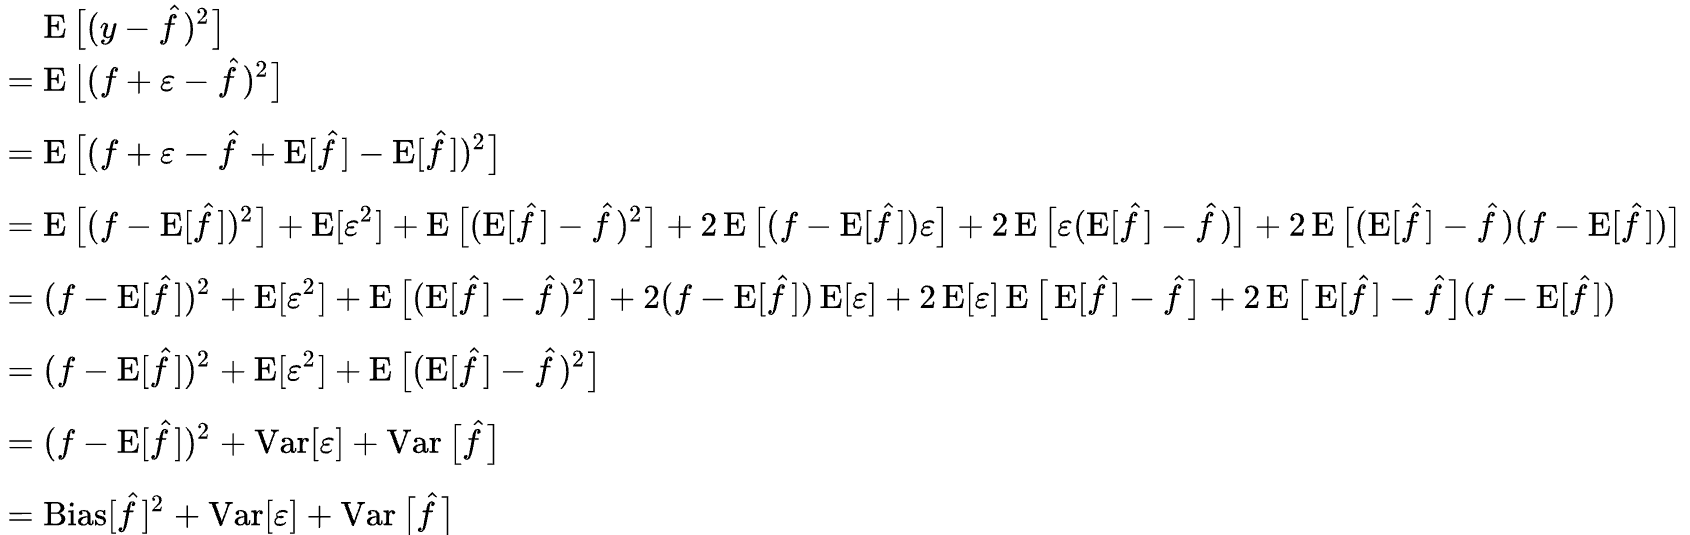
\includegraphics[scale=0.25]{b-v-tradeoff.png}
\\
% \subsection*{Regularization}
% \item{\textbf{Regularization:}}
\textbf{Regularization: } 
Can be viewed as MAP estimation with a prior. Ridge: $\beta \sim \mathcal{N}(0, \frac{\sigma^2}{\lambda I})$; Lasso: $p(\beta_i) = \frac{\lambda}{4 \sigma^2}exp(-|\beta|\frac{\lambda}{2\sigma^2})$ (Laplace, no closed-form solution since $l_1$ norm is not differentiable, more sparse estimations since the gradient of regularization does not shrink as Ridge)
\\
\textbf{Bayesian LR: } 
% \subsection*{Bayesian LR}
% \item{\textbf{Bayesian LR:}}
Assume $\epsilon \sim \mathcal{N}(0, \sigma^2 I)$, $\beta \sim \mathcal{N}(0, \wedge^{-1})$, $p(\beta|Y,X,\sigma^2, \wedge) = \mathcal{N}((X^TX+\sigma^2\wedge)^{-1}X^TY, \sigma^2(X^TX+\sigma^2 \wedge)^{-1})$ \\
Bayesian LR is a special case of Gaussian Processes with linear kernel $k(x, x') = x^T\wedge^{-1} x'$
        % -*- root: Main.tex -*-
\section{Gaussian Processes}
% \subsection*{Prediction with GP}
\textbf{Prediction with GP: } 
% \item{\textbf{Prediction with GP:}}
$p(y_{n+1}|x_{n+1}, X, y) = \mathcal{N}(\color{red}{k(x_{n+1}, X)^T(k(X, X)+\sigma^2 I)^{-1}}\color{red}{y}$,
$\color{blue}{k(x_{n+1} x_{n+1})+$\\$\color{blue}{\sigma^2-k(x_{n+1}, X)^T(k(X,X)+\sigma^2I)^{-1}}k(x_{n+1}, X)}$$)$
% \subsection*{Kernels}
\\
\textbf{Kernels: } 
% \item{\textbf{Kernels:}}
Properties: 1) $k(x, x') = k(x', x)$ 2) $x^TKx \geq 0 \forall x$ 3) $k(x, x') = \phi(x)\phi(x')$; Composition: addition, multiplication, scaling, $k(x,x') = f(k_1(x,x')) = f(x)k_1(x,x')f(x')$ for positive polynomial or exponential $f$; Constructions: 1) $k(x, x') = k_1(x, x') + k_2(x, x')$, Proof: $\exists$ symmetric gram matrices $K_1, K_2$ s.t. $x^TK_1x, x^TK_2x \geq 0 \Rightarrow x^TKx = x^T(K_1+K_2)x \geq 0$ \\
2) $k(x, x') = k_1(x, x')k_2(x, x')$, Proof: $k_1(x, x')k_2(x, x') = \Sigma_{i,j}(f_i(x)g_j(x))(f_i(x')g_j(x')) = \Sigma_{i,j}h_{i,j}(x)h_{i,j}(x') = \phi(x)\phi(x')$ \\
3) $k(x, x') = exp(k_1(x, x'))$, Proof: 
$\sum_{i=1}^{m}\frac{k_1(x, x')^r}{r!} \rightarrow k(x, x')$ as m $\rightarrow \infty$ \\
4) RBF: $k(x, x') = exp(-\frac{1}{2\gamma^2}||x-x'||_2^2) = exp(-\frac{1}{2\gamma^2}||x||_2^2)exp(\frac{1}{\gamma^2}x^Tx')exp(-\frac{1}{2\gamma^2}||x'||_2^2)$ \textcolor{red}{(larger bandwidth $\color{red}{\gamma} \rightarrow$ smoother curves)}
        % -*- root: Main.tex -*-
\section{Ensemble Methods}
\textbf{Bagging: } 
% \subsection*{Bagging (Bootstrapping + Aggregating)}
% $\mathbb{E}[(y - b^{(M)}(x))^2] \leq \mathbb{E}[(y - b(x))^2]$; 
% Proof: 
$\mathbb{E}[(y - b^{(M)}(x))^2] = bias^2(b^{(M)}(x)) + var(b^{(M)}(x)) = bias^2(b(x)) + \frac{1}{M}var(b(x)) \leq \mathbb{E}[(y - b(x))^2]$; Random Forests chooses m random features at each splitting step (i.d. base models). Randomized feature selection induces implicit regularization; no overfitting
\\
% \subsection*{AdaBoost}
\textbf{AdaBoost: } 
$b^{(0)} = 0, w_i^{(0)} = \frac{1}{n}$; 1) $b^{(t)} = min_{\beta}\Sigma_{i}w_{i}^{(t)}\mathbb{I}\{b(x_i)\neq y_i\}$ 2) Evaluate $err_t$ 3) $\tilde{\alpha_t} = \frac{1}{2}log(\frac{1-err_t}{err_t})$, $b^{(t)}= b^{(t-1)} + \tilde{\alpha_t}b^{(t)}$ 4) $w_i^{(t+1)} = w_i^{(t)}exp(-\tilde{\alpha}_ty_ib^{(t)})$ 5) Renormalize $w^{(t+1)}$; Output $\sum(\tilde{\alpha_i}(b^{i}(x))$ \\
Forward stagewise additive modeling:
Proof of 3): $\mathbb{E}[f(x)] := \mathbb{E}[exp(-yf(x))] = P(Y=1|X = x)exp(-f(x))+P(Y=-1|X = x)exp(f(x))$\\
$\frac{\partial \mathbb{E}[f(x)]}{\partial f(x)} = 0 \Rightarrow f^*(x) = \frac{1}{2}\frac{P(Y=1|X = x)}{P(Y=-1|X = x)}$; Proof of 1): $min_{\alpha>0, b\in\mathcal{H}} \sum_i \mathcal{L}(y_i, \alpha b(x_i) + f_{t-1}(x_i) = min_{\alpha, b}\sum_i w_i^{(t)} exp(-\alpha y_i b(x_i))= \min_{\alpha, b}\sum_{i, y_i \neq b(x_i)}w_i^{(t)}e^\alpha + (\sum_iw_i^{(t)}e^{-\alpha} - \sum_{i, y_i \neq b(x_i)}w_i^{(t)}e^{-\alpha})$ ; $w_i^{(t)} = exp(-y_if_{(t-1)}(x_i))$
\\
\textbf{Gradient Boosting: } 
% \subsection*{Gradient Boosting}
$\hat{f}_0(x) = min_{h}\Sigma_{i=1}^{n}(y_i - h(x_i))^2$; 1) $g_t(x_i) = [\frac{\partial \mathcal{L}(y_i, f(x_i))}{\partial f(x_i)}]_{f=\hat{f}_{t-1}(x_i)}$ 2)$h_t = min_h \Sigma_i (-g_t(x_i) - h(x_i))$ 3)$\beta_t = min_{\beta}\Sum_i \mathcal{L}(y_i, \hat{f}_{t-1}(x_i)+\beta h_t(x_i))$ 4)$\hat{f}_{t}(x) = \hat{f}_{t-1}+\beta_t h_t (x)$; Output $\hat{f}_{t}$;
% Adaboost is GB with $\mathcal{L}(y, \hat{y}) = exp(-y\hat{y})$
% \subsection*{Differences between Bagging and Boosting}
% Bagging: randomized, give same importance to all models; Boosting: deterministic, weights weak learners acc. to performances

	% -*- root: Main.tex -*-
\section{Convex Optimization \& SVMs}
% \subsection*{Duality}
% \item{\textbf{Duality:}}
\textbf{Duality: } Primal: $min_{\omega} f(\omega)$ s.t. $g_{i}(\omega) = 0$ and $h_{j}(\omega) \leq 0$
Dual: $max_{\lambda, \alpha}\theta(\lambda, \alpha)$ s.t. $\alpha_{j} \geq 0$
\\
Weak duality: $\theta(\lambda, \alpha) = inf_{\omega \in \mathbb{R}^{d}} \mathcal{L}(\omega, \lambda, \alpha \color{red}{\geq 0)}$ $\leq \mathcal{L}(\omega^{*}, \lambda, \alpha) = f(\omega^{*}) + \sum_{i}\lambda_{i}g_{i}(\omega^{*})$ $\color{red}{(= 0)}$ $+ \sum_{j}\alpha_{j}h_{j}(\omega^{*}) \color{red}{(\leq 0)}$ $\leq f(\omega^{*})$
\\
Slater's condition (check if strong duality holds): 
$\exists \omega$ s.t. $g_i(\omega) = 0, h_i({\omega}) \color{red}{<}$ $0$ $\forall i, j$ \\
Strong Duality (if Slater's holds, convex $f$, non-convex $g$, linear $h$):
1) $\omega^{*} = min_{\omega} \mathcal{L}(\omega, \lambda^{*}, \alpha^{*})$
2) Complementary slackness: $\alpha_{j}h_{j}(\omega^{*}) = 0$, $\forall j$

% \subsection*{SVM (linearly separable case)}
% \item{\textbf{Linearly separable SVM:}}
\textbf{Linearly separable SVM: } 
Primal: $max_{w, w_{0}} 2m(w, w_{0}) = \frac{|w^{T}x^{+} - w^{T}x^{-}|}{||w||} = max_{w, w_0} \frac{2}{||w||} = min_{w, w_0} \frac{1}{2}||w||^2$ for \textcolor{red}{random} $x^{+}, x^{-}$; $y_i(w^{T}x_{i}+w_{0}) \geq 1, \forall i$
\\
Slater's: take $(\gamma w, \gamma w_0)$, $\gamma y_i(w^{T}x_{i} + w_{0}) > 1$
\\
Dual: $\theta(\alpha)$ = $min_{w, w_0}\mathcal{L}(w, w_0, \alpha)$ s.t. $\alpha_i \geq 0, \forall i$ = $min_{w, w_0}\frac{1}{2}||w||^2 + \sum_{i}\alpha_i(1 - y_i(w^T x_i + w_0)) \Leftrightarrow max_{\alpha}-\frac{1}{2}\sum_{ij}\alpha_i \alpha_j y_i y_j x_{i}^{T}x_{j} + \sum_{i}\alpha_i$ ($\sum_{i}\alpha_i y_i = 0$; $w^{*} = \sum_{i}\alpha_i y_i x_i$; $w_{0}^{*} = -\frac{1}{2}({w^{*}}^{T}x^{+} - {w^{*}}^{T}x^{-})$)
\\
Compl. slack.: $\alpha_i^{*}(1 - y_i({w^{*}}^{T} + w_{0}^{*})) = 0$ \Rightarrow $\alpha_{i}^{*} = 0  \Rightarrow w^{*}$ is a sparse comb. of support vectors \\
% \subsection*{SVM (not linearly separable)}
% \item{\textbf{Linearly inseparable SVM:}}
\textbf{Linearly inseparable SVM: } 
Primal: $min_{w, w_0, \xi} \frac{1}{2}||w||^2+C\sum_{i}\xi_{i}$; $y_i(w^{T}x_{i}+w_{0}) \geq 1 - \xi_{i}$; $\xi_{i} \geq 0$; \textcolor{red}{larger} $\color{red}{C}$ \textcolor{red}{means narrower margin, fewer neglected samples, and fewer support vectors.}
\\
Dual: 
$L(w,w_0,\xi,\alpha,\beta)=\frac{1}{2}w^Tw + C\sum_{i=1}^n\xi_i - \sum_{i=1}^{n}\beta_i\xi_i -\sum_{i=1}^{n} \alpha_i(y_i(w^T\phi(x_i) + w_0) -1+\xi_i)$; $0 \leq \alpha_i$ $\color{red}{\leq C}$; $\xi_{i}^{*} = max(0, 1 - y_i({w^{*}^{T} x_i + w_{0}^{*}}))$
\\
% \subsection*{SVM Kernelization}
% \item{\textbf{Kernelization:}}
\textbf{Kernelization: } 
Dual: $max_{\alpha}-\frac{1}{2}\sum_{ij}\alpha_i \alpha_j y_i y_j \phi(x_{i})^{T}\phi(x_{j}) + \sum_{i}\alpha_i$; ${w^{*}}^{T}\phi(x) = \sum_{i} \alpha_{i}^{*}y_i$\sout{$\phi(x_{i})^{T}\phi(x)$}$k(x_i, x)$ \\
% TODO: kernel separation
% \subsection*{Extensions}
% \item{\textbf{Extensions:}}
\textbf{Extensions: } 
SVM Regression: $\epsilon$-sensitive loss: $max(0, |y - f(x)| - \epsilon)$; Primal: $min_{w, \xi, \hat{\xi}} ||w||^{2} + C \sum_{i}(\xi_{i} + \hat{\xi}_{i})$ s.t. $(w^T x_i + w_0) - y_i \leq \epsilon + \xi_i$, $y_i - (w^T x_i + w_0) \leq \epsilon + \hat{\xi}_{i}$, $\xi_{i}, \hat{\xi}_{i} \geq 0$; Dual: $max_{\alpha, \hat{\alpha}}\sum_i (\hat{\alpha} - \alpha)y_i - \epsilon\sum_i (\hat{\alpha} + \alpha) - \frac{1}{2}\sum_{i, j}(\hat{\alpha}_{i} - \alpha_{i})(\hat{\alpha}_{j} - \alpha_{j})x_i x_j$ s.t. $0 \leq \alpha_i, \hat{\alpha}_{i} \leq C$, $\sum_{i, j}(\hat{\alpha}_{i} - \alpha_{i}) = 0$, $\forall i$;
Multi-class SVM: Constraint: $\forall y \in \{1, ..., M\}$, $\forall x_i \in X$, $(w_{y_i}^{T}x_i + w_{y_i, 0}) - max_{y \neq y_i}(w_{y}^{T}x_i + w_{y, 0}) \geq 1 - \xi_i$; Structural SVM: Constraint: $w^T \Phi(y_i, x_i) - max_{y \neq y_i}[\Delta(y, y_i) + w^T \Phi(y, x_i)] \geq -\xi_i$, $\forall x_i \in X$
        % -*- root: Main.tex -*-
\section{Deep Learning \& Generative Models}
% \subsection*{Robbins-Monro Method}
% \item{\textbf{Robbins-Monro Method:}}
\textbf{Robbins-Monro Method: } 
$X_{n+1} = X_{n} - \alpha_n (f(x_n) + \gamma_n)$; Conditions: 1) $lim_{n\rightarrow \infty}\alpha_n = 0$ (convergence) 2) $\sum_{n=1}^{\infty}\alpha_n = \infty$ (slow enough to find root) 3) $\sum_{n=1}^{\infty}\alpha_n^{2} < \infty$  (bounded variance); Proof:
$x_{n+1} - x_0 = x_n - x_0 - \alpha_n (f(x_n) + \gamma_n) \Leftrightarrow \mathbb{E}[(x_{n+1} - x_0)] = \mathbb{E}[(x_{n} - x_0)] - 2\alpha_n \mathbb{E}[(x_{n+1} - x_0)(f(x_n)+\gamma_n)] + \alpha_n^2 \mathbb{E}[f^2(x_n)+2f(x_n)\gamma_n+\gamma_n^2] = \mathbb{E}[(x_{n} - x_0)] + \alpha_n^2 \mathbb{E}[(x_n - x_0)f(x_n)] - 2\alpha_n\mathbb{E}[\gamma_n^2]$; Iterate n-1 times to reduce $x_n$ s.t. $\mathbb{E}[(x_{n+1} - x_0)] - \mathbb{E}[(x_1 - x_0)] \leq (b + \sigma^2) \sum_{i=1}^{n-1}\alpha_i^2 - 2\sum_{i=1}^{n-1}\alpha_i\mathbb{E}[(x_i - x_0)f(x_i)]$; LHS bounded from below \& RHS $\rightarrow -\infty$ iff $(x_i - x_0)f(x_i) \geq 0 \Rightarrow lim_{n\rightarrow \infty} P(x_n = x_0) = 1$.
\\
\textbf{Optimality for step size: } 
% Update rule derivation:
$f(x_n + \Delta x) = f(x_n) + \nabla f(x_n)^T\Delta x + \frac{1}{2}\Delta x^T H \Delta x$; Since $\Delta x = x_{n+1} - x_n = -\alpha_n \nabla f(x_n)$, $f(x_{n+1}) = f(x_n) - \alpha_n \nabla f(x_n)^T\nabla f(x_n) + \frac{1}{2}\alpha_n^2 \nabla f(x_n)^T H \nabla f(x_n)$;
Assume $\frac{\partial}{\partial \alpha_n}f(x_{n+1}) = \frac{\partial}{\partial \alpha_n}f(x_0) = 0 \Leftrightarrow \alpha_n  = \frac{\nabla f^T \nabla f}{\nabla f^T H \nabla f} = H^{-1}$
\\
% \subsection*{SGD}
% \item{\textbf{SGD:}}
\textbf{SGD: } 
Nesterov Momentum: $y_{n+1} = x_n + \beta(x_n - x_{n-1})$; $x_{n+1} = y_{n+1} - \alpha_n \nabla f(y_{n+1})$ for $\beta > 0$; SGD with Momentum: $x_{n+1} = y_{n+1} - \alpha_{n} \nabla f_{I(n)}(y_{n+1})$ with $I(n) \sim \text{Unif}\{1, ..., n\}$; Sign SGD: $x_{n+1} = x_n - \alpha_n sign(\nabla f_{I(n)}(x_n))$; Mini-batch: $x_{n+1} = x_n - \alpha_n \frac{1}{B}\sum_{i \in B}^n \nabla f_i(x_n)$; Unbiased grad: $\mathbb{E}_{I(n)}[\nabla f_{I(n)}] = \frac{1}{n}\sum_{i=1}^{n}\nabla f_i(x) = \nabla f(x)$
\\
\textbf{VAEs: } 
% \subsection*{VAEs}
% \item{\textbf{VAE:}}
Problem: $max_{\theta} p_{\theta}(x) = \int p_{\theta}(z)p_{\theta}(x|z)dz$ is intractable; Solution: define encoder $q_{\theta}(z | x)$ that approximates $p_{\theta}(z|x)$; $log p_{\theta}(x) = \mathbb{E}_{z \sim q_{\theta}(z|x_i)}[log p_{\theta}(x_i)] = \mathbb{E}_z[log\frac{p_{\theta}(x_i|z)p_{\theta}(z)}{p_{\theta}(z|x_i)}\frac{q_{\theta}(z|x_i)}{q_{\theta}(z|x_i)}] = \mathbb{E}_z[log p_{\theta}(x_i | z)] - \mathbb{E}_z[log\frac{q_{\theta}(z|x_i)}{p_\theta(z)}] + \mathbb{E}_z[log\frac{q_{\theta}(z|x_i)}{p_\theta(z|x_i)}] = $\\
$\color{red}{\mathbb{E}_z[log\frac{q_{\theta}(z|x_i)}{p_\theta(z)}] - KL(q_{\theta}(z|x_i) || p_{\theta}(z))}$ $ + KL(q_{\theta}(z|x_i) || p_{\theta}(z|x_i))\geq \color{red}{\mathcal{L}(x_i; \theta, \phi)}$ \textcolor{red}{(ELBO)}\\
\textbf{HVAEs: }Hierarchical latent vectors, top-down shared model with learnable mean and variance to keep long-range data correlations and avoid posterior collapse 
\\
\textbf{GANs: } 
% \subsection*{GANs}
% Generative network tries to fool the discriminator by generating fake data G(z) from noise z; Discriminator tries to distinguish between real and fake data; 
Objective: $\color{red}{min_G}\color{blue}{max_D}$\\$\color{blue}{\{\mathbb{E}_{x\sim p_{data}(x)}[log D(x)]}$$+$$\color{red}{\mathbb{E}_{z\sim p(z)}[log(1-D(G(z)]\}}$ \\
This loss is essentially 2 KL divergences. At early stages, the 2 distributions don't overlap substantially, which leads to \textcolor{red}{vanishing gradient}. Solution: Wasserstein Distance $WG_r(p_1, p_2) = (\mathbb{E}_{x\sim p_1, y\sim p_2}[||x-y||^r])^{\frac{1}{r}}$ \\
\textbf{Extracting representations invariant from domains: }
Conditional GANs: $D \subseteq W \times X \times y$ 1) $E: X \rightarrow Z$ 2) $F: Z \rightarrow [0,1]^y$ 3) $D: Z \times y \rightarrow [0,1]^W$ Objective: $\color{red}{min_{E,F}}$ $\color{blue}{max_D}$ $\color{red}{\mathbb{E}_X[CE(p(y|x), \hat{p}_{E(X)}(\cdot))]}$ $-$ $\color{blue}{\lambda \mathbb{E}_{X,y}[CE(p_{w|x,y}, \hat{p}_{E(X), y}(\cdot))]}$\\
Maximum-mean discrepency: Goal: view representations from 2 domains as 2 samples from the same distribution. 
$MMD(p, q) = sup_{f \in \mathcal{F}}(\mathbb{E}_{X\sim p}[f(X)] - \mahbb{E}_{y\sim q}[f(y)])^2 \approx sup_{f \in \mathcal{H}_0}(\sum_i w_i \mathbb{E}[x_i] - \sum_i w_i \mathbb{E}[y_i]) = sup_{f \in \mathcal{H}_0}(w^T(\mathbb{E}[x^i])-w^T(\mathbb{E}[y^i])) = sup_{f \in \mathcal{H}_0}\langle f, \mu_p-\mu_q \rangle = ||\mu_p - \mu_q||^2 = \mathbb{E}[\sum_i \phi_i(x_1)\phi_i(x_2) - 2\sum_i \phi_i(x) \phi_i(y) + \sum_i \phi_i(y_1)\phi_i(y_2)]$; Objective: $min_{E,F}\mathcal{L}_C(E,F)+\lambda \hat{\mathcal{L}}_{MMD}(E)$
\\
\textbf{Diffusion Models: } 
% \subsection*{Diffusion Models}
$Z_i = \beta_i z_{i-1} + \beta_i \epsilon$, $\epsilon \sim \mathcal{N}(0, I)$, $q(z_i|z_{i-1}) = \mathcal{N}(z_i|\beta_i z_{i-1}, \beta_i I)$; $q(z_t | x) = q(z_t|z_{t-1}) ... q(z_1|x) = \mathcal{N}(z_t|\beta_t z_{t-1}, \beta I) ... \mathcal{N}(z_t|\beta_1 x, \beta_1 I) = \mathcal{N}(z_t|\sqrt{\tilde{\alpha_t}}x, (1-\tilde{\alpha_t})I)$, where $\tilde{\alpha_t} = \prod_s(1-\beta_s)$; Forward posterior: $q(z_{t-1}|z_t, x) = \mathcal{N}(z_{t-1}|\tilde{\mu}_t(z_t, x), \tilde{\beta}_tI)$, where $\tilde{\mu}_t = \frac{\sqrt{\tilde{\alpha}_{t-1}}\beta_t}{1 - \tilde{\alpha}_{t}}x + \frac{\sqrt{1-\beta_t}(1-\tilde{\alpha}_{t-1})}{1 - \tilde{\alpha}_{t}}z_t$, $\tilde{\beta_t} = \frac{1-\tilde{\alpha}_{t-1}}{1 - \tilde{\alpha}_{t}}\beta_t$; New ELBO: $\mathbb{E}[logp(x|z_1)] - KL(q(z_n|x)||p(z_n)) - \sum_i\mathbb{E}[KL(q(z_{i-1}|z_i, x)||p(z_{i-1}|z_i))]$

% \subsection*{Kiefer-Wolfowitz} 
% Conditions: 1) $lim_{n\rightarrow \infty}\alpha_n = lim_{n\rightarrow \infty}c_n = 0$ 2) $\sum_{n=1}^{\infty}\alpha_n = \infty$ 3) $\sum_{n=1}^{\infty}(\frac{\alpha_n}{c_n})^{2} < \infty$
% \\
% \subsection*{Optimality for step size}
% \item{\textbf{Optimal step size:}}
        % -*- root: Main.tex -*-
\section{Non-parametric Bayesian Inference}
\textbf{BI for multivariate Gaussian: } $p(x^*|X) = \int p(x^*|\theta)p(\theta|X)d\theta = \mathbb{E}_{\theta \sim p(\cdot | X)}[p(x^*|\theta)] \approx \frac{1}{M}\sum_t p(x^*|\theta^{(t)})$ where $\theta^{(t)}\sim p(\cdot | X)$; $\mu \sim \mathcal{N}(m_0, V_0), \Sigma \sim IW(S_0, v_0) \Rightarrow \mu | \Sigma, X \sim \mathcal{N}(m_p, V_p), \Sigma | \mu, X \sim IW(S_p, v_p)$ Gibbs sampling: For semi-conjugate priors, iteratively resample acc. to tractable cond. dist. n times. The update does not need to be in exact order for l-dim and first M samples are discarded. \\
\textbf{BI for GMM: } Dirichlet distribution (DP) on $\pi$: $Dir(\pi|\alpha) = \frac{\Gamma(\sum_i \alpha_i)}{\prod_i \Gamma(\alpha_i)} \prod_i \pi_i^{\alpha_i - 1}, \sum_i \pi_i = 1$ \\
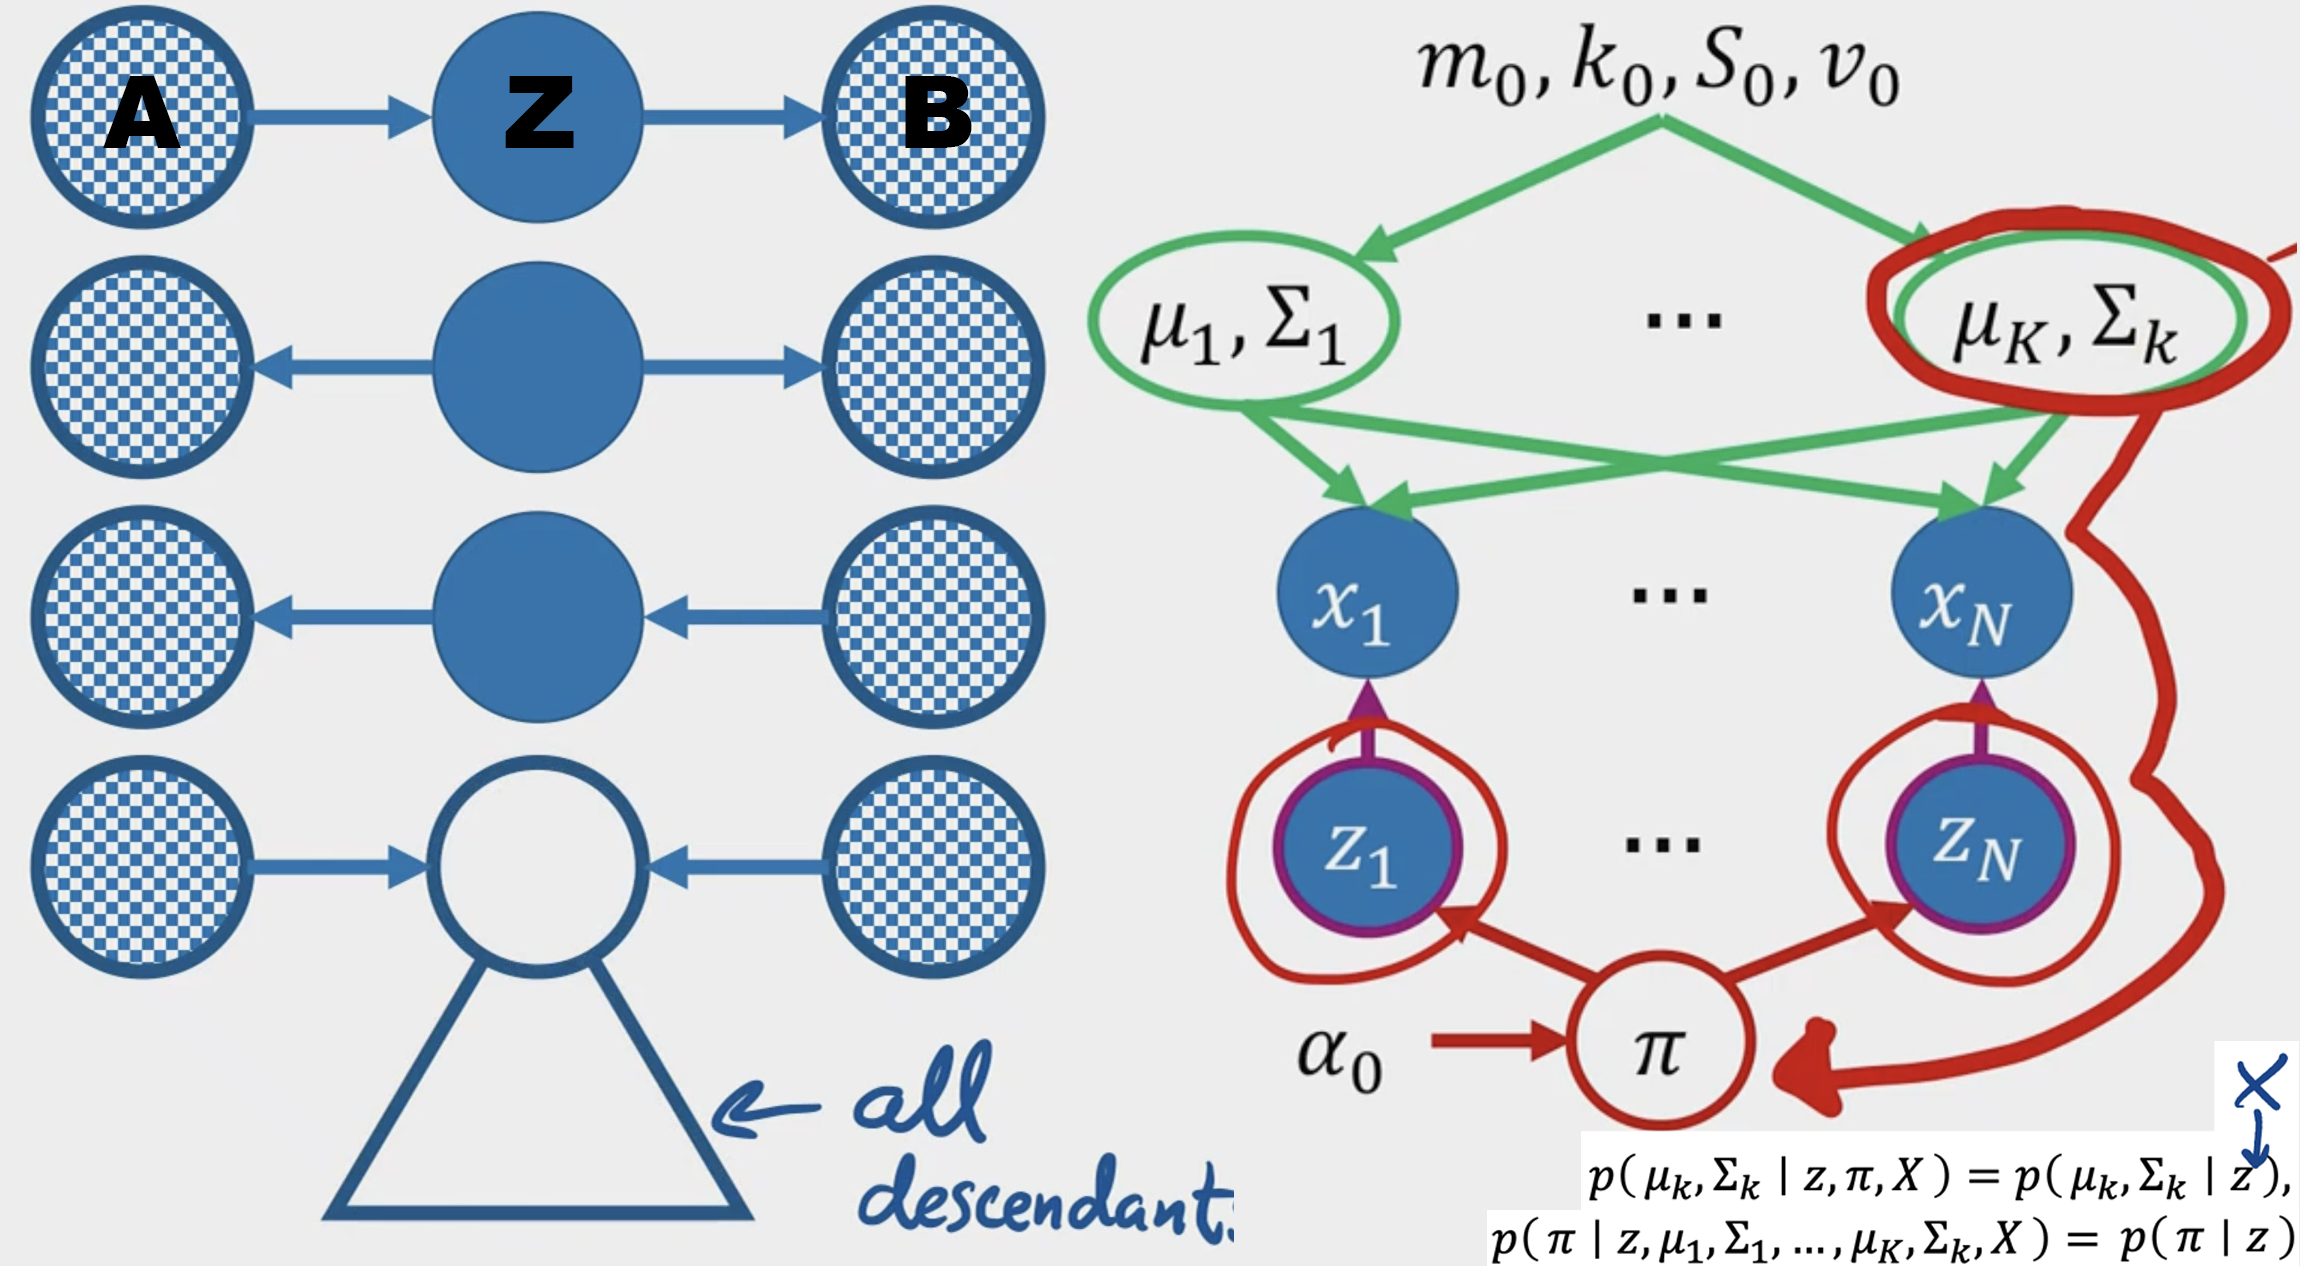
\includegraphics[scale=0.125]{d-separation.png}\\
If every path from variable A to B is blocked by d-separation Z, then A and B are independent conditioned on Z.\\
Collapsed Gibbs sampling: first sample z: $p(z_i = k | z_{-i} = \zeta, X) \propto p(z_i = k | z_{-i} = \zeta)p(X|z_i=k, z_{-i}=\zeta) \propto p(z_i = k | z_{-i} = \zeta)p(x_i|X_{-i}, z_i=k, z_{-i}=\zeta)p(X_{-i}|z_i=k, z_{-i}=\zeta) \propto p(z_i = k | z_{-i} = \zeta)p(x_i | \{x_j: j \leq N_{i \neq j}, z_j = k\})const$; \\
Rao-Blackwellization:
% $\mathbb{E}_{\theta, Z}[f(\theta, Z) | Z] \approx \frac{1}{M}\sum_i \mathbb{E}_{\theta}[f(\theta, z^{(i)}]$, $ z^{(i)}\sim p_z \approx \frac{1}{M}\sum_i f(\theta^{(i)}, z^{(i)})$, $\theta^{(i)}\sim p_{\theta}(\cdot | z^{(i)})$; 
$Var_Z[\mathbb{E}_{\theta}[f(\theta, Z)|Z]] = \mathbb{E}_Z[(\mathbb{E}_{\theta, Z}[f(\theta, Z)] - \mathbb{E}_{\theta'}[f(\theta', Z)])^2] = \mathbb{E}_Z[(\mathbb{E}_{\theta'}[\mathbb{E}_{\theta, Z}[f(\theta, Z)] - f(\theta', Z)])] \leq \mathbb{E}_Z[\mathbb{E}_{\theta'}[(\mathbb{E}_{\theta, Z}[f(\theta, Z)] - f(\theta', Z))^2]] = \mathbb{E}_{Z, \theta'}[(\mathbb{E}_{\theta, Z}[f(\theta, Z)] - f(\theta', Z))^2] = Var_{\theta', Z}[f(\theta', Z)]$ \\
\textbf{BI for non-parametric GMMs: }
% Prior: $\mu_k, \Sigma_k \sim NIW(...), \pi \sim GEM(\alpha), \alpha > 0$; 
Sampling prior: 1) Draw $\pi$ from $GEM(\alpha)$ with Stick-breaking Process: $\pi_1 = \beta_1 \sim Beta(1, \alpha)$, $\pi_{i, i\geq 2} = \prod_{j < i}(1-\beta_j)\beta_i$;
2) Chinese Restaurant Process (metaphor of DP, draw z directly): \\
$p(z_n=k) = $ \begin{cases}
      n_k/(\alpha+n-1), \text{for existing k} \\
      \alpha/(\alpha+n-1), \text{for leftmost empty k}
    \end{cases} \\
$z_1,...,z_n$ are not independent but exchangable. Proof: $p(z_1=k_1, ..., z_n = k_n) = \prod_i p(z_i=k_i|z_1=k_1, ..., z_n=k_n) = \prod_i \frac{f(\alpha, k_i)}{\alpha+i-1} = \prod_i\frac{f(\alpha, k_{\pi^{-1}(i)}}{\alpha+i-1} = p(z_{\pi(1)} = k_1,...,z_{\pi(n)} = k_n)$;
% 3) Dirichlet Process \\
% $(G(T_1), ..., G(T_m)) \sim Dir(\alphaH(T_1), ..., \alphaH(T_m))$ \\
Asymptotics of the expected \# of distinct samples drawn / expected \# of occupied tables in CRP: $S(n) = \sum_k \frac{\alpha}{\alpha+k-1} \geq I(n) = \int_{1}^{n+1}\frac{\alpha}{\alpha+x-1}dx = \alpha(ln(\frac{\alpha+n}{\alpha}))$
\\
DeFinetti’s Theorem: any exchangeable distribution admits a mixture model, $p(X_1 = x_1, ..., X_n = x_n) = \int \prod_i p(x_i|\theta)p(\theta)d\theta$

        % -*- root: Main.tex -*-
\section{PAC Learning}
Algorithm $\mathcal{A}$ can learn $c \in \mathcal{C}$ if $\exists poly(\cdot,\cdot,\cdot)$, s.t. (1) $\forall$ dist. D on X and (2) $\forall \epsilon \in [0,\frac{1}{2}], \delta \in [0,\frac{1}{2}]$, $\mathcal{A}$ outputs $\hat{c} \in H$ given a sample of size at least $poly(\frac{1}{\epsilon},\frac{1}{\delta}, size(c))$ s.t. $p_{Z\sim D^n}(\mathcal{R}(\hat{c}) \leq \epsilon + inf_{c\in \mathcal{C}}\mathcal{R}(c)) \geq 1 - \delta$; $\mathcal{A}$ is an efficient PAC algorithm if it runs in polynomial of $\frac{1}{\epsilon}$ and $\frac{1}{\delta}$. \\
$\mathcal{C}$ is (efficiently) PAC-learnable from $\mathcal{H}$ if there is an algorithm $\mathcal{A}$ that learns
$\mathcal{C}$ from $\mathcal{H}$. \\
\textbf{Rectangle Problem: } $n \geq \frac{4}{\epsilon}ln\frac{4}{\delta}$, suffices to prove $p(\mathcal{R}(\hat{R})\leq \epsilon) \geq p(\hat{R}IG) \geq 1-4exp(-\frac{n\epsilon}{4})$; Proof: $p(\text{¬} \hat{R}IG)\leq \sum_l \prod_i p(x_i \notin T_{l}^{\epsilon}) = 4(1-\frac{\epsilon}{4})^n \leq 4exp(-\frac{n\epsilon}{4})$; Generalization: for $n \geq \frac{1}{\epsilon}(log|\mathcal{H}|+log\frac{1}{\delta})$, $\hat{R}(\hat{h}) = 0 \Rightarrow$ 1) prove $|\mathcal{H}|(1-\epsilon)^n \leq \delta$; 2) prove $p(\hat{R}(\hat{h}) \geq \epsilon) \leq |\mathcal{H}|(1-\epsilon)^n$: $p(\mathcal{R}(\hat{h}) \geq \epsilon) \leq p(\exists h \in \mathcal{H}: \hat{R}(h) = 0 \text{ and } \mathcal{R}(h) \geq \epsilon) \leq \sum_{h\in \mathcal{H}} p(\hat{R}(h) = 0 | \mathcal{R}(h) \geq \epsilon) p(\mathcal{R}(h) \geq \epsilon) \leq \sum_{h} p(\hat{R}(h) = 0 | \mathcal{R}(h) \geq \epsilon) \leq \sum_{h} (1-\epsilon)^n$

\textbf{VC Dimension: } $VC(\mathcal{C})$ = max dimension $n$ s.t. $\exists S \subseteq X, |S| = n$ and S can be shattered \textcolor{red}{(any subset is bounded)} by $\mathcal{C}$; e.g. $VC(\text{intervals}) = 2$. \\
\textbf{Hoeffding's Theorem: } 
$p(S_n - \mathbb{E}_XS_n \geq t) \geq exp(-\frac{2t^2}{\sum_i (b_i - a_i)^2})$; Proof: 1) $p(x \geq t) = p(exp(sX) \geq exp(st)) \leq \frac{\mathbb{E}_X [exp(sX)]}{exp(st)}$; 2) $p(S_n - \mathbb{E}_XS_n \geq t) \leq e^{-st}\mathbb{E}_X[exp(s\sum_i (X_i - \mathbb{E}X_i))] = e^{-st}\prod_i\mathbb{E}_{X_i}[exp(s(X_i-\mathbb{E}X_i))] \leq e^{-st}\prod_iexp(s^2(b_i-a_i)^2/8)$, $s = \frac{4t}{\sum_i(b_i-a_i)^2}$
\\
\textbf{VC Inequality (distribution independent): } For finite $\mathcal{C}$, $p(\mathcal{R}(\hat{c}_n^*) - inf_{c \in \mathcal{C}}(\mathcal{R}(c)) \geq \epsilon) \leq p(\mathcal{R}(\hat{c}_n^*) - \hat{\mathcal{R}}(\hat{c}_n^*) + \hat{\mathcal{R}}(\hat{c}_n^*) - \mathcal{R}(c^*) \geq \epsilon) \leq p(2sup_{c}|\hat{\mathcal{R}}_n(c) - \mathcal{R}(c)| > \epsilon)$
% ; For infinite $\mathcal{C}$: $\leq 9n^{VC_\mathcal{C}}exp(-\frac{n\epsilon^2}{32})$; 
% For finite $\mathcal{C}$: 
$\leq \sum_{c \in \mathcal{C}}p(|\hat{\mathcal{R}}_n(c) - \mathcal{R}(c)| > \epsilon) \leq 2|\mathcal{C}|exp(-2n\epsilon^2) \Rightarrow R(c)$ \textcolor{red}{exp.} $ \leq \hat{R}_n(c) $ \textcolor{red}{emp.} $ + \sqrt{\frac{ln |\mathcal{C}| - ln(\delta / 2)}{2n}}$ \textcolor{red}{var.}
% , using Hoeffding's: $p(S_n - \mathbb{E}_XS_n \geq t) \geq exp(-\frac{2t^2}{\sum_i (b_i - a_i)^2})$ for $b_i = 1, a_i = 0$
	
% -*- root: Main.tex -*-


\end{multicols*}
\end{document}